\documentclass{project-logbook}


\CreateMaintainer{Maya Toitovna}{mtoitovna}{Mars Center for Outstanding Developments}
\CreateContributor{fc}{Frank Chalmers}{fchalmers}{Mars Institute of Technology}
\CreateContributor{ac}{Ann Clayborne}{aclayborne}{Mars Laboratory for Great Achievements}
\CreateContributor{ab}{Arkady Bogdanov}{abogdanov}{Mars University of Fundamental Research}


\SetProjectHeaderName{The very fancy project}
\SetProjectTitle{The title of the project}
\SetProjectSubtitle{The subtitle of the project}

\SetInstitutionLogo{figures/institution-logo.pdf}
\SetProjectSummary{Here you can add a brief summary of your project such that someone can quickly see what it is about, do not spend more than two lines on it.}

\begin{document}
\title{CinC-2016 Logbook}

\MakeFrontPage


\section*{Introduction} % (fold)
\label{sec:introduction}
\PrintContributorsList
\begin{tip}
In this section one should introduce what the research is abLout, in a high level so you can do a simple explanation of the topic and the research challenges that you are facing.
\end{tip}

During the cardiac cycle, the heart firstly generates the electrical activity and then the electrical activity causes atrial and ventricular contractions. This in turn forces blood between the chambers of the heart and around the body. The opening and closure of the heart valves is associated with accelerations-decelerations of blood, giving rise to vibrations of the entire cardiac structure (the heart sounds and murmurs). These vibrations are audible at the chest wall, and listening for specific heart sounds can give an indication of the health of the heart. The phonocardiogram (PCG) is the graphical representation of a heart sound recording. Figure \ref{fig:PCG_ECG} illustrates a short section of a PCG recording.

Then all the contributors: {\GetAllContributorKeys{Name: \ContributorName{#1} }

\begin{figure}[h]
    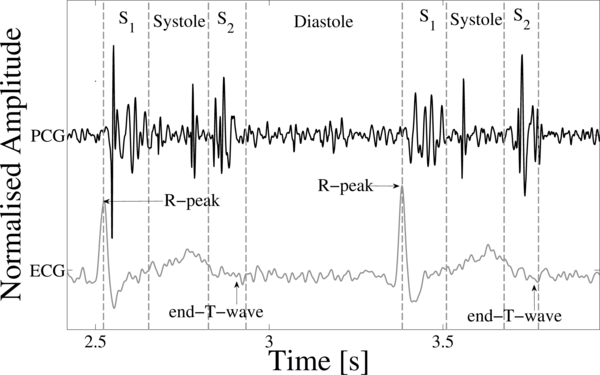
\includegraphics[width=0.6\textwidth]{figures/PCG_ECG}
    \centering
    \caption{A PCG (center tracing), with simultaneously recorded ECG (lower tracing) and the four states of the PCG recording; S1, Systole, S2 and Diastole.}
    \label{fig:PCG_ECG}
\end{figure}

The objective of the challenge is to create a model is able to correctly discriminate between the two classes given just the PCG recordings. Challenges include:

\begin{itemize}
    \item Data is subject to temporal variations due to variations in the heart rate.
    \item Inter-patient differences make difficult a learn a model that generalizes well across patients.
    \item Differences introduced by heterogeneity in the collection of the recordings can render a classifier trained on one population useless when applied to another
\end{itemize}

% section introduction (end)

\section{Dataset and Preprocessing} % (fold)
\label{sec:dataset_and_preprocessing}

\begin{tip}
In most Machine Learning research projects you will be using some kind of samples from a Dataset to learn a model. Thus it is extremely important that you carefully describe the dataset and why you believe is a good dataset for the project and what type of preprocessing are you going to apply
\end{tip}

Early approaches failed to build a reliable model due to lack of a large enough data set, so this challenge provides the largest dataset to this day. Heart sound recordings were sourced from several contributors around the world, collected at either a clinical or nonclinical environment, from both healthy subjects and pathological patients. The Challenge training set consists of five databases (A through E) containing a total of 3,126 heart sound recordings, lasting from 5 seconds to just over 120 seconds.

A main problem found when working with these recordings is the strong similarity between the records coming from the same population  as well as the strong class imbalance of roughly 6:1 of Normal to Abnormal.

Table \ref{tab:populations} summarizes the sizes of the different populations as well as their class imbalance


\begin{table}[ht]
    \centering
    \begin{subtable}{0.48\textwidth}
        \centering
        \begin{tabular}{*{5}{r}}
            {}  & \multicolumn{1}{c}{$A$} & \multicolumn{1}{c}{$N$} & \multicolumn{1}{c}{$S$} & \multicolumn{1}{c}{$A/S$} \\
            \midrule
            a & 292 & 117   & 409   & 0.714 \\
            b & 104 & 386   & 490   & 0.212 \\
            c & 24  & 7     & 31    & 0.774 \\
            d & 28  & 27    & 55    & 0.509 \\
            e & 183 & 1958  & 2141  & 0.085 \\
            \midrule
            & 631 & 2495 & 3126 & 0.202 \\
        \end{tabular}
        \caption{Training Set}
    \end{subtable}
    %
    \begin{subtable}{0.48\textwidth}
        \centering
        \begin{tabular}{*{6}{r}}
            {}  & \multicolumn{1}{c}{$A'$} & \multicolumn{1}{c}{$N'$} & \multicolumn{1}{c}{$S'$} & \multicolumn{1}{c}{$A'/S'$} & $S'/S$ \\
            \midrule
            a & 40  & 40    & 80    & 0.5   & 0.20 \\
            b & 49  & 49    & 98    & 0.5   & 0.20 \\
            c & 4   & 3     & 7     & 0.57  & 0.23 \\
            d & 5   & 5     & 10    & 0.5   & 0.18 \\
            e & 53  & 53    & 106   & 0.5   & 0.05 \\
            \midrule
            & 151 & 150 & 301 & 0.50 & 0.10 \\
        \end{tabular}
        \caption{Validation Set}
    \end{subtable}
    
    \caption{Population properties $A \equiv$ Abnormal, $N\equiv$ Normal, $S\equiv A+N$}
    \label{tab:populations}
\end{table}

\subsection{Preprocessing} % (fold)
\label{sub:preprocessing}

There is a high heterogeneity since it was compiled in different environments with diverse systems and devices. The DTW affinity between representative heartbeats is completely biased if we do not apply any kind of preprocessing.

To prevent this a simple zero mean unit variance normalization approach is used to get closer distances. Nevertheless with a reasonable $\upsigma  = 10^{2.5}$ we can note that the population distances are still there except less noticeable.

\begin{equation}
    x_i' \gets \frac{x_i-\bar{x}}{\upsigma}
\end{equation}
\begin{equation}
    \bar{x} = \frac{1}{N}\sum_{i=1}^{N} x_i \qquad \upsigma^2 = {\frac{1}{N}\sum_{i=1}^{N} (x_i-\bar{x})}
\end{equation}

All the provided records were sampled at $f_s = \SI{2}{\kilo\Hz}$. The segmentation algorithm resamples them\footnote{Resampling = Low Pass Filter + Downsampling by M. The filter will have $\omega_c = \pi/N$ to prevent aliasing} to $ f_s' = \SI{1}{\kilo\Hz}$.
\begin{tipt}{Strike-through}
 Often you will be wrong on your assumptions, but do not throw them away completely, just cross them out in case you need them later using the \texttt{\textbackslash sout} command and it will look like \sout{this} or \texttt{\textbackslash soutthick} command and it will look like \soutthick{this}
\end{tipt}

\sout{Medoid computation is perfomed at $f_s'' = f_s'/5 = \SI{200}{\kilo\hertz}$ to speed computation. Simple analysis was performed to check that the features extracted from these 200Hz-medoids were approximately the same as the ones extracted from the  1khz-medoids.}

\soutthick{Downsampling can be seen as a problem of information loss in the frequency spectrum. If the frequency content $f > f_s/(2N)$ is mostly empty for $N$ when we downsample by said $N$ we will only be losing information in that range.}

\begin{tipt}{TODOs}
You will often have pending tasks that you need to track. This research journal allows you to include both high and low priority todos that will be summarized in a list at the end of the file. Use the commands \texttt{\textbackslash hightodo} and \texttt{\textbackslash lowtodo}, including a date is recommended for tracking purposes.

Note: define your \texttt{userId} in the preamble
\end{tipt}

\hightodo{\Contributorid{hs}}{ 2016-05-23 : Compute the error between mode-downsampled segmentation state vectors at 1000 Hz and state vectors computed at 400 Hz. This needs to be performed to check that the segmentation algorithm is not overfitted to 1000Hz. If error is significant, retrain segmentation at 400 Hz or use 1000 just for segmentation (if Matlab 2016a improvements are true there should be no problem)}

\lowtodo{\Contributorid{hp}}{ 2016-05-27 : Do DRYRUN with new Matlab 2016a and check the segmentation quota }

% subsection preprocessing (end)

% section dataset_and_preprocessing (end)
\newpage
\section{Methods} % (fold)
\label{sec:methods}

\subsection{Algorithms} % (fold)
\label{sub:algorithms}

\begin{tip}
Sometimes the most straightforward way to explain a procedure is just to give it in a algorithmic format, it takes a little time but it will force you to go thorugh the steps and you will most likely be able to reuse it on you paper.
Note: You will need to have \texttt{\textbackslash ALGORITHMStrue} in the preamble to enable algorithms
\end{tip}

\begin{algorithm}
\caption{Euclid’s algorithm}\label{alg:euclid}
\begin{algorithmic}[1]
\Procedure{Euclid}{$a,b$}\Comment{The g.c.d. of a and b}
\State $r\gets a\bmod b$
\While{$r\not=0$}\Comment{We have the answer if r is 0}
\State $a\gets b$
\State $b\gets r$
\State $r\gets a\bmod b$
\EndWhile\label{euclidendwhile}
\State \textbf{return} $b$\Comment{The gcd is b}
\EndProcedure
\end{algorithmic}
\end{algorithm}


% subsection algorithms (end)

\subsection{Code} % (fold)
\label{sub:code}

\begin{tip}
If the algorithm is to vague and you feel like you need the source code you can also insert it. You can put LaTeX code inside by using \texttt{<@ @>} delimiters and highlight it with \texttt{<| |>} delimiters

Note: you will need to have \texttt{\textbackslash
LISTINGStrue} in the preamble.
\end{tip}

\begin{lstlisting}[style=Python]
def DTW_distance(s1, s2):
	"""
	Function to compute the Dynamic Time Warping in Python between two signals
	"""
	DTW={}

	for i in range(len(s1)):
		DTW[(i, -1)] = float('inf') # By default <@\color{pgreen} $\infty$@>
	for i in range(len(s2)):
		DTW[(-1, i)] = float('inf') # By default <@\color{pgreen} $\infty$@>
	DTW[(-1, -1)] = 0

	for i in range(len(s1)):
		for j in range(len(s2)):
			dist= (s1[i]-s2[j])**2
			<|DTW[(i, j)] = dist + min(DTW[(i-1, j)],DTW[(i, j-1)], DTW[(i-1, j-1)])|>

	return sqrt(DTW[len(s1)-1, len(s2)-1])
\end{lstlisting}

% subsection code (end)
\clearpage
\subsection{Diagrams} % (fold)
\label{sub:diagrams}

\begin{tip}
For simple diagrams I highly recommend learning TiKZ, you will be drawing the diagrams in pure \LaTeX which has a steep learning curve but once you get used to it, it can be quite easy to display and do \texttt{for} loops to draw multiples line at once.

Note: you will need to have \texttt{\textbackslash
TiKZtrue} in the preamble
\end{tip}

\begin{figure}[!h]
\centering
\tikzset{%
  every neuron/.style={
    circle,
    draw,
    minimum size=1cm
  },
  neuron missing/.style={
    draw=none,
    scale=4,
    text height=0.333cm,
    execute at begin node=\color{black}$\vdots$
  },
}

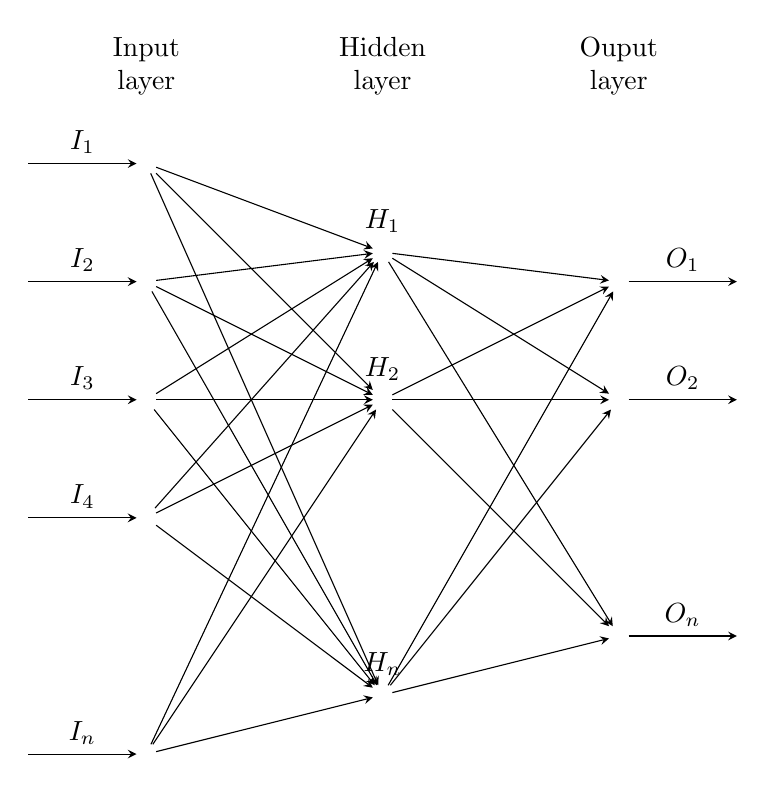
\begin{tikzpicture}[x=1.5cm, y=1.5cm, >=stealth]

\foreach \m/\l [count=\y] in {1,2,3,4,missing,5}
  \node [every neuron/.try, neuron \m/.try] (input-\m) at (0,2.5-\y) {};

\foreach \m [count=\y] in {1,2,missing,3}
  \node [every neuron/.try, neuron \m/.try ] (hidden-\m) at (2,2-\y*1.25) {};

\foreach \m [count=\y] in {1,2,missing,3}
  \node [every neuron/.try, neuron \m/.try ] (output-\m) at (4,1.5-\y) {};

\foreach \l [count=\i] in {1,2,3,4,n}
  \draw [<-] (input-\i) -- ++(-1,0)
    node [above, midway] {$I_\l$};

\foreach \l [count=\i] in {1,2,n}
  \node [above] at (hidden-\i.north) {$H_\l$};

\foreach \l [count=\i] in {1,2,n}
  \draw [->] (output-\i) -- ++(1,0)
    node [above, midway] {$O_\l$};

\foreach \i in {1,...,5}
  \foreach \j in {1,...,3}
    \draw [->] (input-\i) -- (hidden-\j);

\foreach \i in {1,...,3}
  \foreach \j in {1,...,3}
    \draw [->] (hidden-\i) -- (output-\j);

\foreach \l [count=\x from 0] in {Input, Hidden, Ouput}
  \node [align=center, above] at (\x*2,2) {\l \\ layer};

\end{tikzpicture}
\end{figure}

\begin{tip}
However, sometimes you will need more complicated diagrams (or maybe you do not like TiKZ, in that case I recommend a vector drawing tool such as Inkscape which allows \LaTeX \,embedding)
\end{tip}

\begin{figure}[h]
    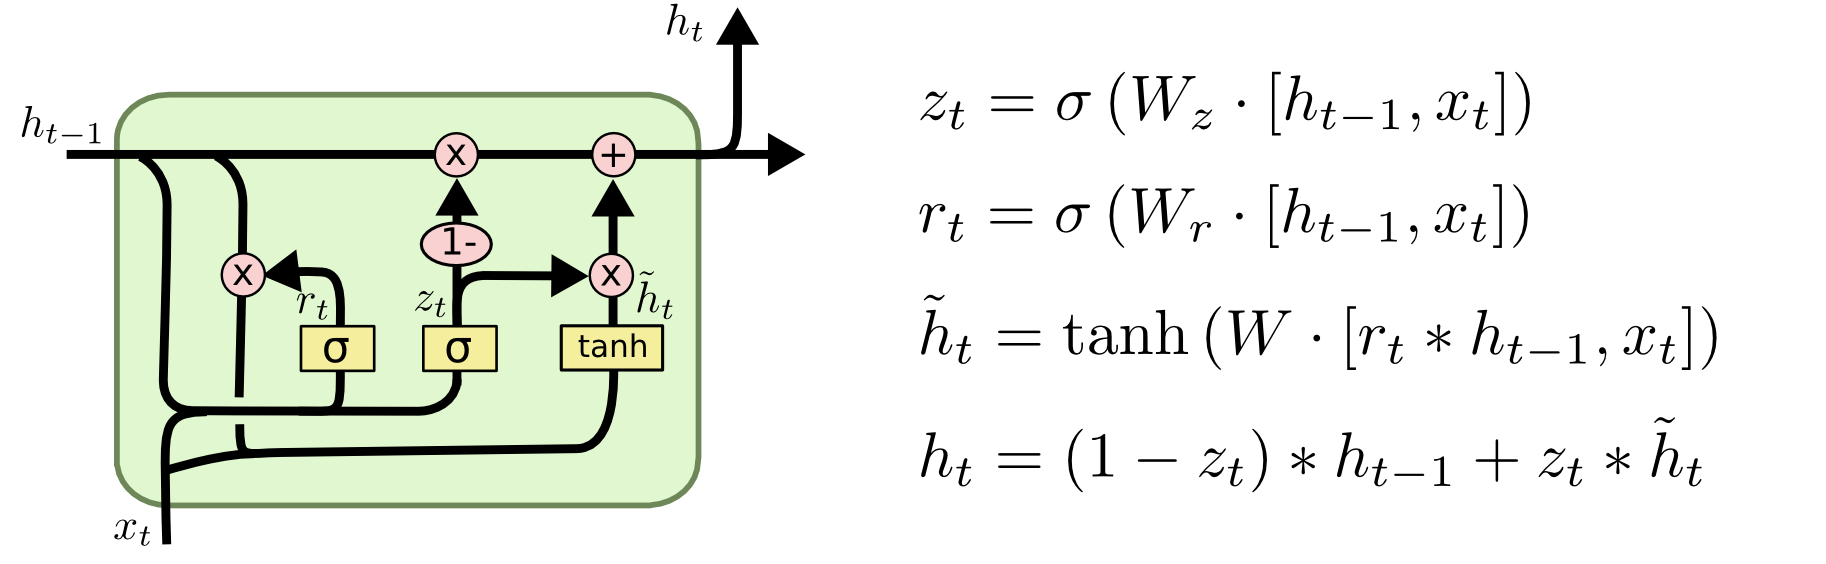
\includegraphics[width=0.9\textwidth]{figures/LSTM}
    \centering
    \caption{Gate Recurrent Unit in a Long Short Term Memory Neural Netwok (GRU-LSTM). \\ \emph{Credit to \url{https://colah.github.io/posts/2015-08-Understanding-LSTMs/}}}
    \label{fig:LSTM}
\end{figure}

% subsection diagrams (end)

% section methods (end)

\section{Results} % (fold)
\label{sec:results}

\subsection{Figures} % (fold)
\label{sub:figures}

\begin{tip}
In general the best way to visualize your results will be some figures, I recommend Python's matplotlib for generating them or R's ggplot2.
\end{tip}

\begin{figure}[htp]
    \centering
    \begin{subfigure}{0.48\textwidth}
        \centering
        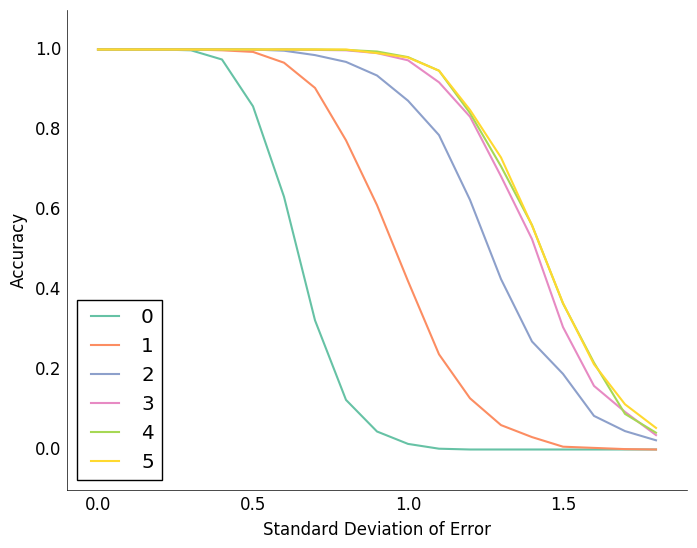
\includegraphics[width=\textwidth]{figures/accuracy_128.png}
        \caption{Average accuracies for 128-bit key}
    \end{subfigure}
    \hspace{.35cm}
    \begin{subfigure}{0.48\textwidth}
        \centering
        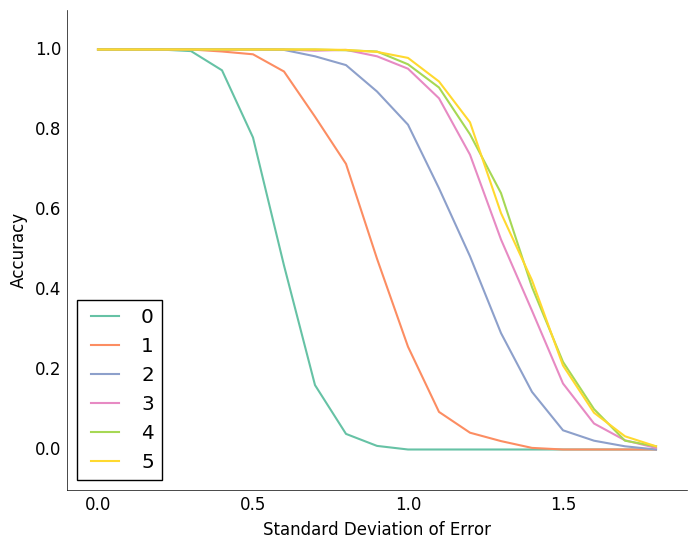
\includegraphics[width=\textwidth]{figures/accuracy_192.png}
        \caption{Average accuracies for 192-bit key}
    \end{subfigure}%

    \vspace{1cm}
    \begin{subfigure}{0.48\textwidth}
        \centering
        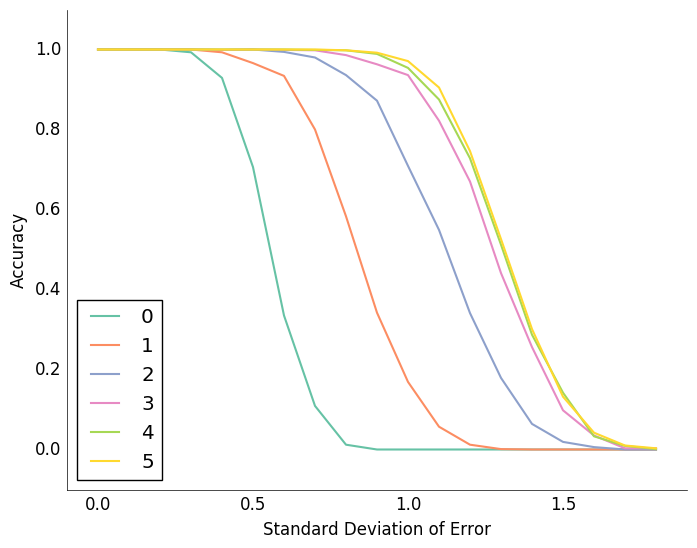
\includegraphics[width=\textwidth]{figures/accuracy_256.png}
        \caption{Average accuracies for 256-bit key}
    \end{subfigure}
    \hspace{.35cm}
    \begin{subfigure}{0.48\textwidth}
        \centering
        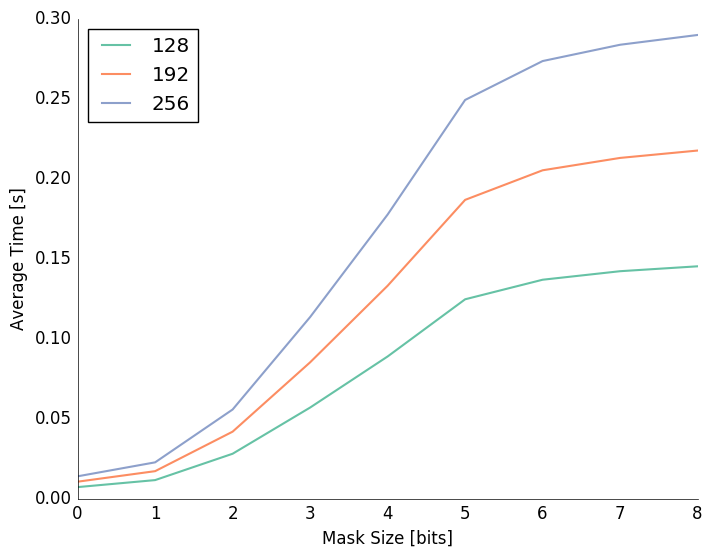
\includegraphics[width=\textwidth]{figures/times.png}
        \caption{Average Runtimes for various mask sizes}
    \end{subfigure}
    \vspace{.25cm}
    \caption{Results of simulation of the LMS algorithm with correction}
    \label{fig:plots}
\end{figure}

% subsection figures (end)

\subsection{Tables} % (fold)
\label{sub:tables}

\begin{tip}
\LaTeX \; booktab environments are really good to showcase and track your results, however they can get fairly messy. My suggestion is to generate them via Python automatically and store the results in either a plain text file or a spreadsheet (there are packages to read spreadsheets with Python)
\end{tip}

\begin{table}[ht]
     \centering
     \begin{tabular}{rrrrrrrrrr}
         $\upsigma \setminus \tau$ & \multicolumn{1}{c}{0} &\multicolumn{1}{c}{1} &\multicolumn{1}{c}{2} &\multicolumn{1}{c}{3} &\multicolumn{1}{c}{4} &\multicolumn{1}{c}{5} &\multicolumn{1}{c}{6} &\multicolumn{1}{c}{7} &\multicolumn{1}{c}{8}\\
          \midrule
         0.0 & 100.0  &100.0  &100.0  &100.0  &100.0  &100.0  &100.0  &100.0  &100.0 \\
         0.2 & 100.0  &100.0  &100.0  &100.0  &100.0  &100.0  &100.0  &100.0  &100.0 \\
         0.4 & 100.0  &100.0  &100.0  &100.0  &100.0  &100.0  &100.0  &100.0  &100.0 \\
         0.6 & 98.6  &100.0  &100.0  &100.0  &100.0  &100.0  &100.0  &100.0  &100.0 \\
         0.8 & 84.7  &99.5  &100.0  &100.0  &100.0  &100.0  &100.0  &100.0  &100.0 \\
         1.0 & 28.1  &98.3  &99.9  &100.0  &100.0  &100.0  &100.0  &100.0  &100.0 \\
         1.2 & 1.3  &88.7  &99.4  &99.9  &99.8  &99.9  &100.0  &99.9  &100.0 \\
         1.4 & 0.0  &57.1  &96.2  &99.3  &99.0  &99.3  &99.4  &99.8  &99.7 \\
         1.6 & 0.0  &18.6  &81.2  &93.0  &93.7  &94.8  &95.6  &92.3  &93.3 \\
         1.8 & 0.0  &2.4  &42.8  &67.0  &70.1  &72.1  &69.0  &69.1  &68.6 \\
         2.0 & 0.0  &0.1  &9.0  &23.1  &24.5  &26.9  &28.2  &27.3  &27.3 \\
         \midrule
          $t$(ms) &27.92 &40.23 &77.30 &157.27 &252.05 &342.18 &381.46 &399.85 &413.72\\
     \end{tabular}
     \caption{Performance of the algorithm for 128-bit key and with multiple readings per key}
     \label{tab:error_128_avg}
 \end{table}

% subsection tables (end)

% section results (end)




%----------------------------------------------------------------------------------------
%   REFERENCE LIST
%----------------------------------------------------------------------------------------
\clearpage
\appendix
\section{Resources}
\begin{tip}
It is a good idea to record sources that explain concepts or provide tools so the research is both better documented and if someone has to continue with it, there is enough supporting documentation.
\end{tip}
\begin{itemize}
    \item Quick read in DTW and Keogh Lower Bounding

\url{http://alexminnaar.com/time-series-classification-and-clustering-with-python.html}

\url{http://nbviewer.jupyter.org/github/alexminnaar/time-series-classification-and-clustering/blob/master/Time%20Series%20Classification%20and%20Clustering.ipynb}
    \item Parallelizing DTW -- Good article on making a parallel version of DTW. Uses Keogh lower bound not as a linear approximation but as a pruning device.

    \url{https://www.andrew.cmu.edu/user/mmohta/15418Project/finalreport.html}

    \item Deep Learning
    \begin{itemize}
        \item Intro to LSTM

        \url{https://colah.github.io/posts/2015-08-Understanding-LSTMs}
        
        \item Intro to CNN

        \url{https://colah.github.io/posts/2014-07-Conv-Nets-Modular/}

        \item Why are LSTMs are so useful, impressive result in character pattern and syntax learning

        \url{https://karpathy.github.io/2015/05/21/rnn-effectiveness/}
    \end{itemize}
\end{itemize}
\section{References}
\begin{tip}
Do not forget to cite the papers that you are using in your research, this way the \textbf{Previous Work} part in your paper will be infinitely easier to write when the time comes.
\end{tip}
\nocite{*}
\bibliographystyle{alpha}
\bibliography{mybib}
\clearpage
\section{TO DO}
\begin{tip}
Here you will have all your TODOs grouped with anchor links to the parts of the document where they are. Really handy if you do not know where to continue with your project.
\end{tip}
\listoftodos

\end{document}